\documentclass{ltjsarticle}
\RequirePackage{luatex85}
\usepackage[utf8]{inputenc}
\usepackage[dvipdfmx]{color}
\usepackage{enumerate}
\usepackage{here}
\usepackage{amsthm}
\usepackage{amsfonts}
\usepackage{amsmath}
\usepackage{amssymb}
\usepackage{latexsym}
\usepackage{ytableau}
\usepackage{docmute}
\usepackage{mathtools}
\usepackage{xr}
\usepackage{tikz}
\usetikzlibrary{intersections, calc, arrows.meta}
\usepackage[all]{xy}
\usepackage{graphics}
\usepackage[luatex]{hyperref}
%\usepackage{pxjahyper}



\theoremstyle{definition}
\newtheorem{defin}{定義}[subsection]
\newtheorem{theo}[defin]{定理}
\newtheorem{cor}[defin]{系}
\newtheorem{prop}[defin]{命題}
\newtheorem{lemm}[defin]{補題}
\newtheorem{notice}[defin]{注意}
\newtheorem{eg}[defin]{例}
\newtheorem{fact}[defin]{事実}


\renewcommand{\labelenumi}{(\roman{enumi})}


\newcommand{\invlimit}{\mathop{\lim_{\longleftarrow}}}
\newcommand{\dirlimit}{\mathop{\lim_{\longrightarrow}}}
\newcommand{\ind}{\text{Ind}}
\newcommand{\Hom}{\text{Hom}}
\newcommand{\tr}{\text{tr}}
\newcommand{\id}[1]{\text{id}_{#1}}
\newcommand{\sgn}{\mathrm{sgn}}
\newcommand{\res}[1]{\text{Res}_{#1}}
\newcommand{\generated}[1]{\langle\:#1\:\rangle}
\newcommand{\im}{\text{Im }}
\newcommand{\rank}{\text{rank }}
\newcommand{\del}[2]{\frac{\partial #1}{\partial #2}}
\newcommand{\delsametwo}[2]{\frac{\partial^2 #1}{\partial #2^2}}
\newcommand{\delothertwo}[3]{\frac{\partial^2#1}{\partial#2\partial#3}}
\newcommand{\ddel}[2]{\frac{\partial}{\partial #2}#1}
\newcommand{\ddelsametwo}[3]{\frac{\partial^2}{\partial #2^2}#1}
\newcommand{\ddelothertwo}[3]{\frac{\partial^2}{\partial#2\partial#3}#1}
\newcommand{\simneq}{\not\simeq}
\newcommand{\transpose}[1]{^t\!#1}
\newcommand{\ie}{\text{i.e.}}
\newcommand{\inv}[1]{#1^{-1}}
\newcommand{\real}{\mathbb{R}}
\newcommand{\complex}{\mathbb{C}}
\newcommand{\integer}{\mathbb{Z}}
\newcommand{\quotient}{\mathbb{Q}}
\newcommand{\natnum}{\mathbb{N}}
\newcommand{\proj}{\mathbb{P}}
\newcommand{\affine}{\mathbb{A}}
\newcommand{\tensor}[3]{#1\otimes_#2#3}
\newcommand{\map}[3]{#1:#2\rightarrow#3}
\newcommand{\aut}[2]{\mathrm{Aut}_{#1} (#2)}
\newcommand{\hommoph}[2]{\mathrm{Hom}_{#1}(#2)}
\newcommand{\gl}{\text{GL}}
\newcommand{\End}{\text{End}}
\newcommand{\set}[2]{\left\{\:#1\:\middle|\:#2\:\right\}}
\newcommand{\pmat}[1]{\begin{pmatrix} #1
\end{pmatrix}}
\newcommand{\vmat}[1]{\begin{vmatrix} #1
\end{vmatrix}}
\newcommand{\bmat}[1]{\begin{bmatrix} #1
\end{bmatrix}}
\newcommand{\br}{\vskip\baselineskip}
\newcommand{\Lie}{\text{Lie}}
\newcommand{\Sym}{\text{Sym}}
\newcommand{\Alt}{\text{Alt}}
\newcommand{\ch}{\text{ch}}
\newcommand{\diag}{\text{diag}}
\newcommand{\comb}[2]{_{#1}C_{#2}}
\newcommand{\codim}{\text{codim}\:}
\newcommand{\yd}[1]{\ydiagram{#1}}

\title{aaa}
\author{}
\date{}


\begin{document}
\maketitle

\begin{figure}[H]
  \centering
  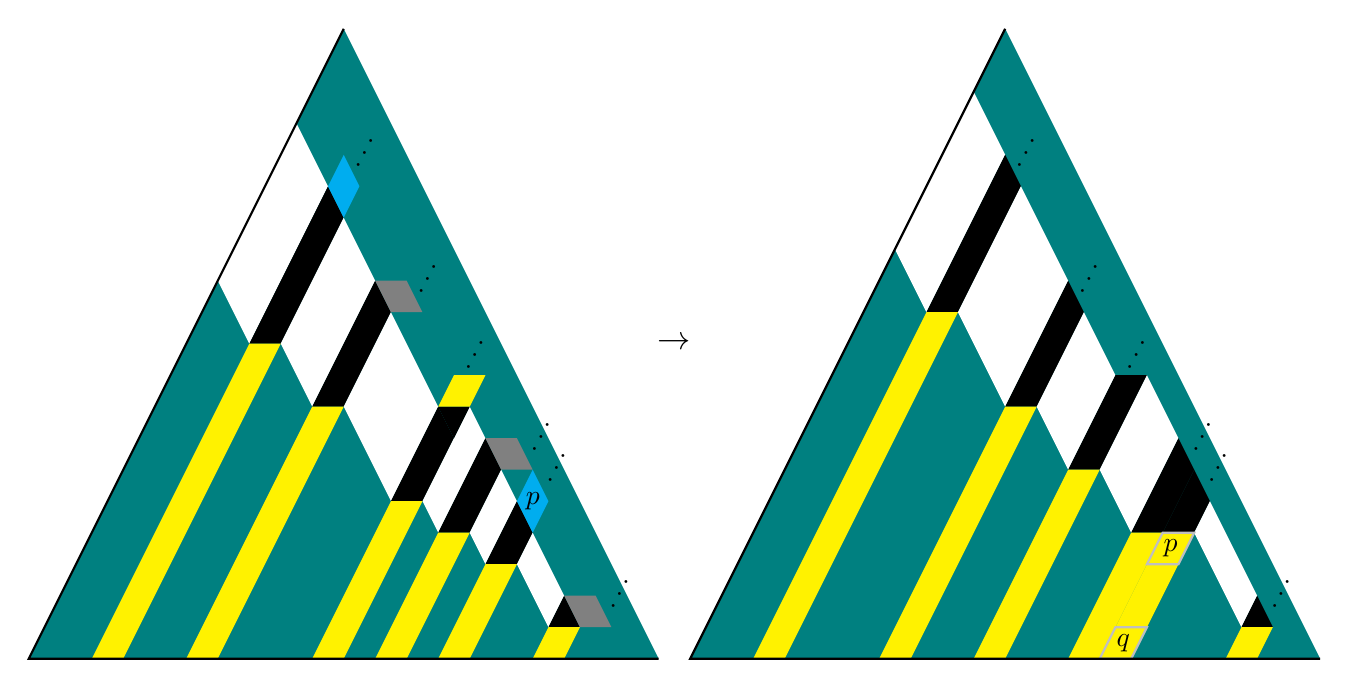
\begin{tikzpicture}[xscale = 0.8, yscale = 0.8]
    \fill[teal] (0,0)--(10,0)--(5,10)--cycle;
    \begin{scope}[xshift=1cm,yshift=2cm]
      \fill[white] (8/4,8/2)-- ++(5/4,5/2)-- ++(1/2,-1)-- ++(-5/4,-5/2)--cycle;
      \fill[black] (15/4,11/2)-- ++(1/4,-1/2)-- ++(-4/4,-4/2)-- ++(-1/2,0)--cycle;

      \fill[white] (16/4,10/2)-- ++(2/4,-2/2)-- ++(-4/4,-4/2)-- ++(-1/2,1)--cycle;
      \fill[black] (18/4,8/2)-- ++(1/4,-1/2)-- ++(-3/4,-3/2)-- ++(-1/2,0)--cycle;

      \fill[white] (19/4,7/2)-- ++(3/4,-3/2)-- ++(-3/4,-3/2)-- ++(-3/4,3/2)--cycle;
      \fill[black] (22/4,4/2)-- ++(1/4,-1/2)-- ++(-2/4,-2/2)-- ++(-1/2,0)--cycle;

      \fill[white] (24/4,4/2)-- ++(1/4,-1/2)-- ++(-3/4,-3/2)-- ++(-1/4,1/2)--cycle;
      \fill[black] (25/4,3/2)-- ++(1/4,-1/2)-- ++(-2/4,-2/2)-- ++(-1/2,0)--cycle;

      \fill[white] (26/4,2/2)-- ++(1/4,-1/2)-- ++(-2/4,-2/2)-- ++(-1/4,1/2)--cycle;
      \fill[black] (27/4,1/2)-- ++(1/4,-1/2)-- ++(-1/4,-1/2)--++(-1/2,0)--cycle;

      \fill[white] (28/4,0)-- ++(2/4,-2/2)-- ++(-1/4,-1/2)-- ++(-2/4,2/2)--cycle;
      \fill[black] (30/4,-2/2)-- ++(1/4,-1/2)-- ++(-1/2,0)--cycle;

  


      \fill[yellow] (10/4,6/2)-- ++(1/2,0)-- ++(-10/4,-10/2)-- ++(-1/2,0)--cycle;
      \fill[yellow] (14/4,4/2)-- ++(1/2,0)-- ++(-8/4,-8/2)-- ++(-1/2,0)--cycle;
      \fill[yellow] (19/4,1/2)-- ++(1/2,0)-- ++(-5/4,-5/2)-- ++(-1/2,0)--cycle;
      \fill[yellow] (22/4,0)-- ++(1/2,0)-- ++(-4/4,-4/2)-- ++(-1/2,0)--cycle;
      \fill[yellow] (25/4,-1/2)-- ++(1/2,0)-- ++(-3/4,-3/2)-- ++(-1/2,0)--cycle;
      \fill[yellow] (29/4,-3/2)-- ++(1/2,0)-- ++(-1/4,-1/2)-- ++(-1/2,0)--cycle;



      \fill[cyan] (15/4,11/2)-- ++(1/4,-1/2)-- ++(1/4,1/2)-- ++(-1/4,1/2)--cycle;
      \fill[gray] (18/4,8/2)-- ++(1/2,0)-- ++(1/4,-1/2)-- ++(-1/2,0)--cycle;
      \fill[black] (22/4,4/2)-- ++(1/2,0)-- ++(-1/4,-1/2)--cycle;
      \fill[yellow] (22/4,4/2)-- ++(1/2,0)-- ++(1/4,1/2)-- ++(-1/2,0)--cycle;
      \fill[gray] (25/4,3/2)-- ++(1/2,0)-- ++(1/4,-1/2)-- ++(-1/2,0)--cycle;
      \fill[cyan] (27/4,1/2)-- ++(1/4,-1/2)-- ++(1/4,1/2)-- ++(-1/4,1/2)--cycle;
      \node at (28/4,1/2) {$p$};
      \fill[gray] (30/4,-2/2)-- ++(1/2,0)-- ++(1/4,-1/2)-- ++(-1/2,0)--cycle;
    \end{scope}


    \node at (-2/5+0.1 + 22/4, 16/2) {\rotatebox{100}{$\ddots$}};
    \node at (-2/5+0.1 + 26/4, 12/2) {\rotatebox{100}{$\ddots$}};
    \node at (-2/5+0.1 + 29/4, 10/2-0.2) {\rotatebox{100}{$\ddots$}};
    \node at (-2/5+0.4 + 32/4, 7/2) {\rotatebox{100}{$\ddots$}};
    \node at (-2/5+0.4 + 33/4, 6/2) {\rotatebox{100}{$\ddots$}};
    \node at (-2/5+0.4 + 37/4, 2/2) {\rotatebox{100}{$\ddots$}};
    \node[font=\large] at (10.25, 5) {$\rightarrow$};

    \draw[thick] (10,0)--(0,0)--(5,10);






    \begin{scope}[xshift=10.5cm]
      \fill[teal] (0,0)--(10,0)--(5,10)--cycle;
    \begin{scope}[xshift=1cm,yshift=2cm]
      \fill[white] (9/4,9/2)-- ++(5/4,5/2)-- ++(1/2,-1)-- ++(-5/4,-5/2)--cycle;
      \fill[black] (16/4,12/2)-- ++(1/4,-1/2)-- ++(-4/4,-4/2)-- ++(-1/2,0)--cycle;

      \fill[white] (17/4,11/2)-- ++(3/4,-3/2)-- ++(-4/4,-4/2)-- ++(-3/4,3/2)--cycle;
      \fill[black] (20/4,8/2)-- ++(1/4,-1/2)-- ++(-3/4,-3/2)-- ++(-1/2,0)--cycle;

      \fill[white] (21/4,7/2)-- ++(2/4,-2/2)-- ++(-3/4,-3/2)-- ++(-2/4,2/2)--cycle;
      \fill[black] (23/4,5/2)-- ++(1/2, 0)-- ++(-3/4,-3/2)-- ++(-1/2,0)--cycle;

      \fill[white] (25/4,5/2)-- ++(2/4,-2/2)-- ++(-3/4,-3/2)-- ++(-2/4,2/2)--cycle;
      \fill[black] (27/4,3/2)-- ++(1/4,-1/2)-- ++(-2/4,-2/2)-- ++(-1/2,0)--cycle;

      \fill[black] (28/4,2/2)-- ++(1/4,-1/2)-- ++(-1/4,-1/2)--++(-1/2,0)--cycle;

      \fill[white] (29/4,1/2)-- ++(3/4,-3/2)-- ++(-1/4,-1/2)-- ++(-3/4,3/2)--cycle;
      \fill[black] (32/4,-2/2)-- ++(1/4,-1/2)-- ++(-1/2,0)--cycle;

  


      \fill[yellow] (11/4,7/2)-- ++(1/2,0)-- ++(-11/4,-11/2)-- ++(-1/2,0)--cycle;
      \fill[yellow] (16/4,4/2)-- ++(1/2,0)-- ++(-8/4,-8/2)-- ++(-1/2,0)--cycle;
      \fill[yellow] (20/4,2/2)-- ++(1/2,0)-- ++(-6/4,-6/2)-- ++(-1/2,0)--cycle;
      \fill[yellow] (24/4,0)-- ++(1/2,0)-- ++(-4/4,-4/2)-- ++(-1/2,0)--cycle;
      \fill[yellow] (26/4,0)-- ++(1/2,0)-- ++(-4/4,-4/2)-- ++(-1/2,0)--cycle;
      \node at (26/4 + 1/8, -1/4) {$p$};
      \node at (23/4 + 1/8, -3/2-1/4) {$q$};
      \draw[lightgray,thick] (26/4,0) -- ++(1/2,0) -- ++(-1/4,-1/2)-- ++(-1/2,0)--cycle;
      \draw[lightgray,thick] (23/4,-3/2) -- ++(1/2,0) -- ++(-1/4,-1/2)-- ++(-1/2,0)--cycle;
      \fill[yellow] (31/4,-3/2)-- ++(1/2,0)-- ++(-1/4,-1/2)-- ++(-1/2,0)--cycle;
    \end{scope}


    \node at (-2/5+0.1 + 22/4, 16/2) {\rotatebox{100}{$\ddots$}};
    \node at (-2/5+0.1 + 26/4, 12/2) {\rotatebox{100}{$\ddots$}};
    \node at (-2/5+0.1 + 29/4, 10/2-0.2) {\rotatebox{100}{$\ddots$}};
    \node at (-2/5+0.4 + 32/4, 7/2) {\rotatebox{100}{$\ddots$}};
    \node at (-2/5+0.4 + 33/4, 6/2) {\rotatebox{100}{$\ddots$}};
    \node at (-2/5+0.4 + 37/4, 2/2) {\rotatebox{100}{$\ddots$}};

    \draw[thick] (10,0)--(0,0)--(5,10);
    \end{scope}
  \end{tikzpicture}
  \caption{} \label{weight preserving}
\end{figure}

\end{document}